\documentclass[thesis-solanki.tex]{subfiles}

\ifMain
\externaldocument{thesis-solanki}
\fi
\begin{document}

\chapter{Prototype 1}{\label{proto1}}



\section{About this chapter}

This chapter demonstrates a fairly generic procedure of creating an open embedded domain specific language in
\progLang{Haskell} along with \textit{monadic unification}.
As a proof of concept, the implementation consists of creating a
\progLang{Prolog}-like open language whose unification procedure is
carried out in a monad.


\section{Ideas}
There are four main ideas in this chapter
that we work with to develop a working implementation of embedded \progLang{Prolog}
using the concepts mentioned above.

\begin{enumerate}
\item \progLang{Prolog}

The language itself has a number of sub components.
The ones relevant to this thesis are:
\begin{enumerate}
\item Language, the syntax, semantics.

\item Database, or the knowledge base where the rules are stored.

\item Unification

\item
  \progLang{Prolog} has to satisfy a list of goals while maintaining variable bindings and choice points.
  For a non empty list of list of goals, it looks through the knowledge base for matching rules and attempts at
  unifying the terms and repeats until all goals have been satisfied.
  If more than one option is available, they are recorded as choice points which are later used for backtracking
  and finding other possible solutions.

\item
  Lastly, the query resolver which combines the unification and search strategy to return a result.
\end{enumerate}

\item \codeLibrary{prolog-0.2.0.1} \cite{prolog-lib}

  One of the existing implementation of \progLang{Prolog} in \progLang{Haskell}, though partial, provides a starting
  point for the implementation as it provides
  certain components to test
  our approach.
  The main components of this library are adopted from \progLang{Prolog} and modified. These are:

\begin{enumerate}
\item the language, adopted from \progLang{Prolog} but trimmed down;

\item the database;

\item the unifier;

\item the Read-Eval-Print Loop (REPL);

\item the interpreter which consists of a parsing mechanism and resembles the query resolver.
\end{enumerate}

\item \codeLibrary{unification-fd} \cite{unification-fd-lib}

This library provides tools for first-order structural unification over general structure types along with mechanisms for a modifiable
generic unification algorithm implementation.

The relevant components are:
\begin{enumerate}
\item the \haskellClass{Unifiable} class;

\item the \haskellConstruct{UTerm} data type;

\item variable implementations:
  \haskellConstruct{STVar} and \haskellConstruct{IntVar};

\item the \haskellClass{Binding} monad; and 

\item Unification (\haskellConstruct{unify} and \haskellConstruct{unifyOccurs}).
\end{enumerate}

\item Prototype 1

  This implementation applies to practice the procedure to create an open language to accommodate types,
  custom variables, quantifiers and logic and recovering primitives while preserving the structure of a
  language commonly defined by a recursive abstract syntax tree.
  The resulting language is then adapted to apply a \progLang{Prolog}-like unification.

The implementation consists of the following components:
\begin{enumerate}
\item an open language,

\item compatibility with the unification library \cite{unification-fd-lib},

\item variable bindings, and

\item monadic unification.

\end{enumerate}
\end{enumerate}

Each of the components are discussed in the following sections.




\section{Prototype architecture}

\begin{figure}[H]
  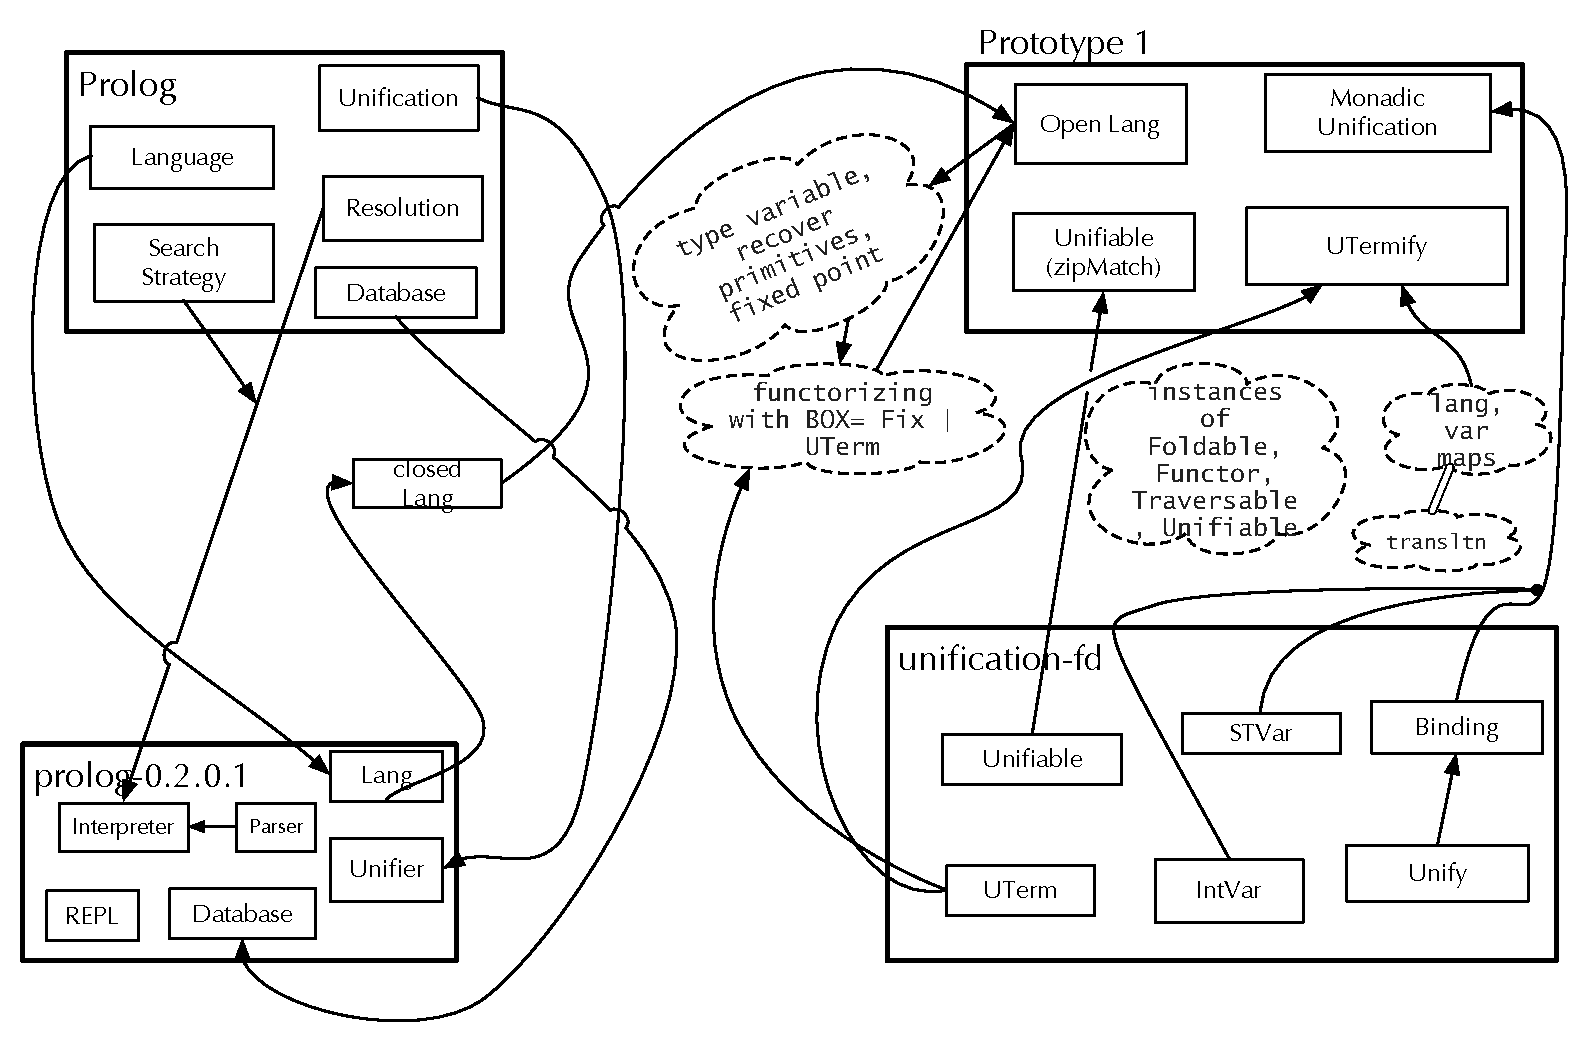
\includegraphics[width=1\textwidth]{Prototype-1.pdf}
  \caption{Architecture of Prototype 1}
  \label{fig:proto1-arch}
\end{figure}
Chapter~\ref{chap:pwp} provides a general description of the working of \progLang{Prolog}.
In this prototype we explore the unification aspect only.  

This prototype demonstrates the process of creating an isomorphic data type to replicate the target language type system while
conforming to the host language.

We create a \progLang{Prolog}-like language using a recursive abstract grammar in \progLang{Haskell} using
\progLang{Haskell}'s  \haskellConstruct{data} statement.
We then convert it to a non-recursive version whose fixed point is isomorphically equivalent to the original.
This gives us a more open implementation which will be discussed in the sections to come.

The rest of the procedure includes managing library compatibility for the language and, more importantly, monadic
unification.

\section{Creating a data type}
%% dgc removed the [H] as it forces a bad page break.
\begin{figure}
  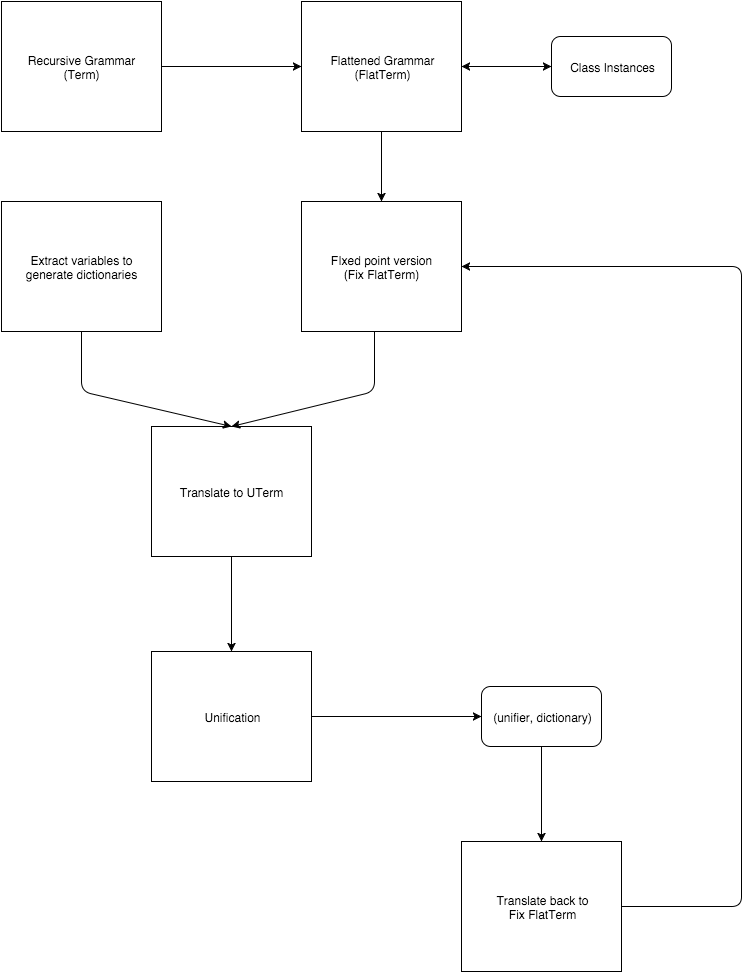
\includegraphics[width=1\textwidth]{prototype_1_implementation_architecture.png}
  \caption{Prototype 1 Implementation architecture}
  \label{fig:proto1-impl-arch}
\end{figure}

To start we need to define an abstract syntax for a \progLang{Prolog}-like language.
Consider the language in Listing~\ref{tab:closed-terms}, which has been adopted from
\cite{prolog-lib}.

\begin{code-list}[H]
\begin{singlespace}
\inputminted{haskell}{haskell-proto1-closed-terms.hs}
\end{singlespace}
  \caption{A classic recursive grammar}
  \label{tab:closed-terms}
\end{code-list}

Even though \textit{Term} has a number of constructors the resulting construct has a single type.
Hence, a binary function would have type
\par
\mint{haskell}|foo :: Term -> Term -> Term|

Listing~\ref{tab:closed-terms} is a classic example of using a recursive data type to define the
abstract syntax of a language.
One of the issues with the datatype in Listing~\ref{tab:closed-terms} is that it is not possible to distinguish the structure of the data from
the data type itself \cite{sheard2004two}.
Moreover, the primitives of the language (see \cite{website:understandingalgebrasfpcomplete})
are not accessible, as the language can have expressions of only one
type, ``\haskellConstruct{Term}''.

\begin{comment}
The solution  would be to add a type constructor split the data type into two levels, a single recursive
data type is replaced by two related data types.
\end{comment}
Consider the code in Listing~\ref{tab:non-recurse}.
\begin{code-list}[H]
\begin{singlespace}
\inputminted{haskell}{haskell-proto1-non-recurse.hs}
\end{singlespace}
  \caption{A flattened (non-recursive) grammar}
  \label{tab:non-recurse}
\end{code-list}

One result of coding as in Listing~\ref{tab:non-recurse} rather than as in Listing~\ref{tab:closed-terms} (lines
6--9) is that the non-recursive type \texttt{FlatTerm} is modular and generic as the structure
\haskellConstruct{FlatTerm} is separate from the type of its subterms
which is \haskellVar{a}.
The above language can be of any type \haskellConstruct{FlatTerm} \haskellVar{a} where \haskellVar{a} can be of any
type at all.
A more accurate way of saying it would be that \haskellVar{a} can be any \textit{kind} in
\progLang{Haskell}.

In type theory, a kind is the type of a type constructor or, less commonly, the type of a higher-order type
operator.
A kind system is essentially a simply-typed \(\lambda\)-calculus `one level up', endowed with a primitive type,
denoted \Verb!*!
and called `type', which is the kind of any (monomorphic) data type
(see \cite{website:kindhaskellwiki}).
Listing~\ref{tab:kindsinhaskell} describes kinds in \progLang{Haskell}.

\begin{code-list}[H]
\begin{singlespace}
\inputminted{haskell}{haskell-proto1-kinds-in-haskell.hs}
\end{singlespace}
\caption{\haskellConstruct{kinds} in \progLang{Haskell}}
\label{tab:kindsinhaskell}
\end{code-list}

Simply speaking we can have something like
\mint{haskell}|FlatTerm Bool|
and a generic function like,
\mint{haskell}|function :: (a -> b) -> FlatTerm a -> FlatTerm b|

One problem remains: how does one represent deep expressions
of the above language, 
for example something of the form,
\mint{haskell}|FlatTerm(FlatTerm (FlatTerm (FlatTerm (....... (a)))))|
and how to represent it generically to perform operations on it, since
\mint{haskell}|(FlatTerm a) != (FlatTerm (FlatTerm a))|

%
because with our original grammar all the expression that could be defined would be represented by a single entity
\haskellConstruct{Term}, no matter how deep they were.

The approach to tackling this problem is to find the ``fixed-point'' of \haskellConstruct{FlatTerm}.
After infinitely many iterations we should get to a fixed point where further iterations make no
difference.
It means that applying one more \haskellConstruct{FlatTerm} would not change anything---%
a \progLang{Haskell} provides fixed-points in two forms, one for data and one for types.

In type constructor form,
\mint{haskell}|newtype Fix f = f (Fix f)|
which we apply to our abstract syntax.

The resulting language is of the form,\endnote{%
  There is a weird \TeX{} problem here jamming lines together.
}
\mint{haskell}|data Prolog = P (Fix FlatTerm) deriving (Show,Eq,Ord)|
%
simply speaking all the expressions resulting from \haskellConstruct{FlatTerm} can be represented  by the type signature \haskellConstruct{Fix FlatTerm}.

A sample function working with such expressions would be of the form,
\mint{haskell}|func :: Fix FlatTerm -> Fix FlatTerm|


Generically speaking, the language can be expanded for additional functionality without changing or modifying the
base structure.
Consider the scenario where the language needs to accommodate additional type of terms. There are two appraoches:

\begin{enumerate}
\item Manually modify the structure of the language, as shown in Listing~\ref{tab:man-enhan-gram}.
  \begin{code-list}[H]
\begin{singlespace}
\inputminted{haskell}{haskell-proto1-man-enhan-gram.hs}
\end{singlespace}
    \caption{A manually enhanced recursive grammar}
    \label{tab:man-enhan-gram}
  \end{code-list}

  This would then trigger a ripple effect throughout the architecture because accommodations need to be made for
  the new functionality.

\item
  The other option would be to \textit{functorize} language like we did by adding a type variable which can be used
  to plug something that provides the functionality into the language.
  Since we needed the fixed point of the language we used \haskellConstruct{Fix} but generically one could add
  custom functionality.
  For instance, using \haskellConstruct{Extended} from Listing~\ref{tab:garfunkle} we have that
  \haskellConstruct{Extended} \haskellConstruct{FlatTerm} is isomorphic to the type defined in Listing~\ref{tab:man-enhan-gram}.
\begin{comment}  
  Consider the following example,

\begin{minted}[linenos]{haskell}
data Box f = Abox | T f (Box f) deriving (.........)
\end{minted}

then something like,
\begin{minted}[linenos]{haskell}
T (Struct 'atom' [Abox, T (Cut 0)])
\end{minted}
\end{comment}
\end{enumerate}



\begin{code-list}[H]
\begin{singlespace}
\inputminted{haskell}{haskell-proto1-garfunkle.hs}
\end{singlespace}
  \caption{The \protect{\haskellConstruct{Extended}} type constructor}
  \label{tab:garfunkle}
\end{code-list}

Figure~\ref{fig:manual-extension} and Figure~\ref{fig:automatic-extension} show the extension of the example in Listing~\ref{tab:closed-terms} using the
manual
and functorized approach respectively.

\begin{figure}[H]
  \centering
  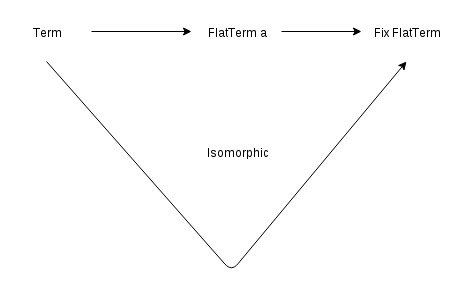
\includegraphics[scale=0.1, width=0.7\textwidth]{extended_data_type_1.png}
  \caption{Manually Extension of data type}
  \label{fig:manual-extension}
\end{figure}

\begin{figure}[H]
  \centering
  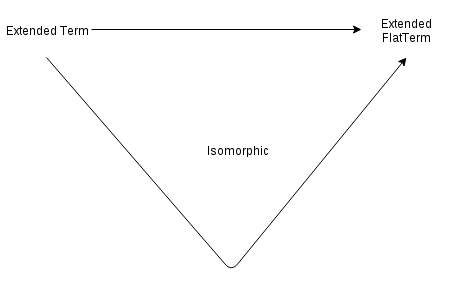
\includegraphics[width=0.7\textwidth, scale=0.1]{extended_data_type_2.png}
  \caption{Automatic Extension of data type}
  \label{fig:automatic-extension}
\end{figure}


\section[Making the language compatible with \protect\codeLibrary{unification-fd}]{Making the language compatible with \newline\codeLibrary{unification-fd}}\label{sec:making-lang-comp}

Our language is now opened up and ready for expansion, but it still needs to conform to the requirements of the
\codeLibrary{unifiication-fd} library (\cite{unification-fd-lib}) for the unification algorithm to work.

The library provides functionality for first-order structural unification over general structure types along with
mutable variable bindings.

In this section we discuss
\begin{enumerate}
\item Functor hierarchy.

\item Required instances the language must have.

\item Mutable variables.

\item Variable bindings.

\item Monadic unification.

\item Replicating \progLang{Prolog} unification in \progLang{Haskell}
\end{enumerate}

Classes in \progLang{Haskell} are like containers with certain properties which can be thought of as functions. When a data type creates an
instance of a class the function(s) can be applied to each element / primitive in the data type.


The data here is the \progLang{Prolog} abstract syntax and the containers are
\haskellClass{Functor}, \haskellClass{Foldable}, and \haskellClass{Traversable}.
Figure~\ref{fig:Functor Hierarchy} shows the relation between the different classes.

\begin{figure}[th]
\centering
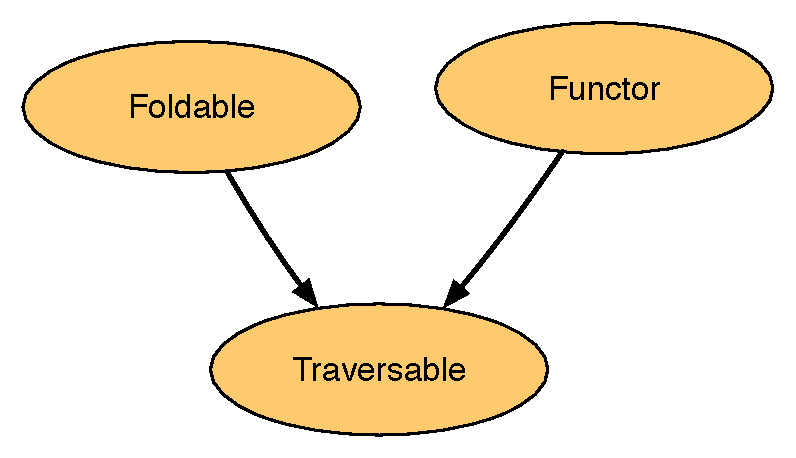
\includegraphics[scale = 0.7]{FunctorHierarchy.pdf}
\caption{Functor Hierarchy (simplified from \cite{website:foldablenadtraversable})}
\label{fig:Functor Hierarchy}
\end{figure}

The \haskellClass{Functor} and \haskellClass{Foldable} instances provide functions for applying map-reduce as described in Chapter~\ref{chap:relatedWork}.
\endnote{%
  Also it is not clear that you are talking about the functional interface to \texttt{map-reduce} rather than the
  large-scale data capabilities.  Perhaps this can be cleared up in Chapter~\ref{chap:relatedWork}.
}
to the data structure.
The primary issue is that at the end of the operation the structure if the data type is lost which would not help
our cause since the result of a query must be a list of substitutions which are essential pairs of language
variable with language values (language constructs).

Enter \haskellConstruct{Traversable}.
It allows reduce whilst preserving the shape of the structure.
We create the necessary instances
as shown in Listing~\ref{tab:flat-term-class-inst}.
\begin{code-list}[H]
  \begin{singlespace}
    \inputminted[linenos,lastline=12]{haskell}{haskell-proto1-class-flat.hs}
  \end{singlespace}
  \caption{\protect\haskellConstruct{FlatTerm} class instances}
  \label{tab:flat-term-class-inst}
\end{code-list}

The above lay the foundation to work with the library.
Coming back to the library, the language must have the \haskellClass{Unifiable} instance.
This works in tandem with the \haskellConstruct{UTerm} data type.
The \haskellConstruct{UTerm} data type captures the recursive structure of logic terms, i.e., given
some functor \(t\) which describes the 
constructors of our logic terms, and some type \(v\) which describes our logic variables, the type
\haskellConstruct{UTerm} \(t\) \(v\) is the
type of logic terms: trees with multiple layers of \(t\) structure and leaves of type \(v\).
The \haskellClass{Unifiable} class gives one step of the unification process.
Just as we only need to specify one level of the ADT (i.e., \Verb!T!) and then we can use the library's \haskellConstruct{UTerm} to generate
the recursive ADT, so too we only need to specify one level of the unification (i.e., \haskellConstruct{zipMatch}) and then we can use
the library's operators to perform the recursive unification.
This is shown in Figure~\ref{tab:zipMatch}.
\begin{code-list}[H]
  \begin{singlespace}
    \inputminted[linenos]{haskell}{haskell-proto1-zip-flat.hs}
  \end{singlespace}
  \vspace*{-0.5\baselineskip}
  \caption{\protect\haskellConstruct{FlatTerm} instance of \protect\haskellConstruct{zipMatch}}
  \label{tab:zipMatch}
\end{code-list}

Unification involves side effects of binding logic variables to terms. To allow and keep track of these effects we use the binding monad
which provides facilities to generate fresh logic variables and perform look ups on dictionaries. By default two logic variable
implementations exist:
\begin{enumerate}
\item The \haskellConstruct{IntVar} implementation uses \haskellConstruct{Int} as the names of variables, and uses an
  \haskellConstruct{IntMap} to keep track of the environment. 

\item The \haskellConstruct{STVar} implementation uses \haskellConstruct{STRef}s, so we can use actual mutation for binding logic
  variables, rather than keeping an explicit environment around.

\end{enumerate}

\begin{comment}
  The library ships with two implementations of logic variables.
  The \markWord{IntVar} implementation uses \markWord{Int} as the names of variables, and uses an \markWord{IntMap}
  to keep track of the 
  environment.
  The \markWord{STVar} implementation uses \markWord{STRefs}, so we can use actual mutation for binding logic variables, rather than
  keeping an explicit environment around.
  This implementation uses \markWord{STVars}.

  Performing unification has the side effect of binding logic variables to terms.
  Thus, we'll want to use a monad in order to keep track of these effects.
  The \markWord{BindingMonad} type class provides the definition of what we need from our ambient monad.
  In particular, we need to be able to generate fresh logic variables, to bind logic variables, and to lookup what
  our logic variables are bound to.
  The library provides the necessary instances for both \markWord{IntVar} and \markWord{STVar}.

  You can provide your own implementations of \markWord{Variable} and \markWord{BindingMonad}.
\end{comment}

%\textbf{Some stuff about Meta syntactic variables can be put in here}

\begin{comment}
The issue with the \haskellConstruct{State monad} is that it can only hold substitutions of a single type \haskellConstruct{State}. For
using several different term datatypes at the same time we need to use the \haskellConstruct{ST monad}. \haskellConstruct{ST monad} 
provides the capability to  create, read and update reference cells of arbitrary type \cite{claessen2000typed} .
\end{comment}

The \haskellConstruct{ST monad} is similar to the \haskellConstruct{IO monad} but is escapable. An \haskellConstruct{ST} action  is of the 
form:

\mint{haskell}|ST s a|

\haskellVar{a} is the return type of the result of the computation in thread \haskellVar{s}. The s keeps references to objects inside the 
\haskellConstruct{ST monad} from leaking to the outside of the \haskellConstruct{ST monad} meaning the actions can only affect their own 
thread. To escape we require:
\mint{haskell}|runST :: forall a. (forall s. ST s a) -> a|

The action \haskellVar{a} must be universal in \haskellVar{s}, meaning the threading association is not known prohibiting to other threads and thus 
\haskellConstruct{runST} is pure \cite{website:stmonadwiki, website:stmonadstackoverflow}. This is the idea behind \haskellConstruct{STVars} which are 
implemented using \haskellConstruct{STRefs}. Hence to use "true mutability" we carry out the computation in the \haskellConstruct{ST monad}.

This implementation uses \haskellConstruct{STVars} and \haskellConstruct{STBindings} to implement the \haskellConstruct{BindingMonad}
but a custom implementation could also be used inside the \haskellConstruct{BindingMonad}.
For our language expressions to be unifiable we must deal with the variables in the expressions being compared.
For that we extract the variables and then convert them into a dictionary consisting of a free variable for each
language variable as shown in Figure~\ref{tab:varsToDictM}.

\begin{code-list}[H]
  \begin{singlespace}
  \inputminted[linenos]{haskell}{haskell-proto1-var-extract.hs}
  \end{singlespace}
  %\vspace*{-1.0\baselineskip}
  \caption{Creating a variable dictionary}
  \label{tab:varsToDictM}
\end{code-list}

A language to \haskellConstruct{STVar} dictionary is only one part of the unification procedure, the terms themselves should be made
compatible for the in built unify procedure to perform look ups for the variables in them.
The dictionary along with the fixed point version flattened of the term, as shown in Figure~\ref{tab:to-UTerm}.
%
\begin{code-list}[H]
  \begin{singlespace}
  \inputminted[linenos]{haskell}{haskell-proto1-utermify-frog.hs}
  \end{singlespace}
  \caption{Conversion to UTerm}
  \label{tab:to-UTerm}
\end{code-list}
%
and for later use to convert them back, as shown in Figure~\ref{tab:from-UTerm}.
%
\begin{code-list}[H]
  \begin{singlespace}
    \inputminted[linenos]{haskell}{haskell-proto1-vtermify-goat.hs}
  \end{singlespace}
  \caption{Conversion from UTerm}
  \label{tab:from-UTerm}
\end{code-list}


The variable dictionaries and \haskellConstruct{UTerm}ified language expressions are unified in the binding monad as shown
in Figure~\ref{tab:unification} and Figure~\ref{tab:unif-driver}.

%
\begin{code-list}
  \begin{singlespace}
    \inputminted[linenos]{haskell}{haskell-proto1-unify-monad.hs}
  \end{singlespace}
  \caption{Unification code}
  \label{tab:unification}
\end{code-list}

\begin{code-list}[H]
  \begin{singlespace}
    \inputminted[linenos]{haskell}{haskell-proto1-unify-driver.hs}
  \end{singlespace}
  \caption{Driver code}
  \label{tab:unif-driver}
\end{code-list}


The final reconversion to return a list of substitutions,
  called \haskellConstruct{f1} in Figure~\ref{tab:unif-driver}, is shown in
  Figure~\ref{tab:vars-extract}.
\begin{code-list}[H]
  \begin{singlespace}
    \inputminted[linenos]{haskell}{haskell-proto1-unify-out.hs}
  \end{singlespace}
  \caption{Variable substitution list extraction}
  \label{tab:vars-extract}
\end{code-list}

\section{Chapter recapitulation}
Recapitulating, this chapter provides the ideas of language modification and monadic unification along with their respective 
implementations. 


\ifMain
\begin{scope}
  \nolinenumbers
  \enotesize
  \par
  \begin{singlespace}
  \setlength{\parskip}{12pt plus 2pt minus 1pt}
  \theendnotes
  \par
  \end{singlespace}
\end{scope}
\unbcbibliography{bibliography}
\fi

\end{document}
